% Ch9 self-study -- "I do / You do" ladder for Zumdahl 9.1, with 9.2-9.3
% as clearly-marked enrichment. Ten figures.
%
% SCOPE DECISION, deliberate: TEXTBOOK-MAP puts Zumdahl 9.2-9.5
% (Molecular Orbital theory) on the SKIP LIST -- it is not on the 2024
% CED. So ladders 1-8 go deep on 9.1, which IS assessed, and MO theory
% appears once, at the end, flagged as enrichment and not examinable.
% Padding the assessed half or expanding the unassessed half would both
% be worse than saying so plainly.
\documentclass{apchem-worksheet}

\apcunitword{Chapter}
\apcunit{9}
\apcunittitle{Covalent Bonding: Orbitals}
\apcdoctitle{Self-Study \textbullet\ Chapter 9, I~do / You~do}
\apcsubtitle{Zumdahl \S9.1 (assessed) $+$ \S9.2--9.3 (enrichment) \textbullet\ PDF pp.\ 455--480}

\begin{document}
\apctitleblock

\begin{apcnote}[How to use these notes --- read this first]
Each skill is a \textbf{ladder}: a fully worked example in the
solid-framed box, then \textbf{four} YOUR TURN questions in the dashed
box --- same skill, new numbers, no help. Work all four before checking
the gray \emph{check:} line; a tracker tick needs all four right first
time.

\textbf{A scope warning that will save you hours.} Zumdahl's
\S9.2--9.5 --- the whole Molecular Orbital chapter, MO diagrams,
bond order from MO counts, homonuclear and heteronuclear diatomics ---
is \textbf{not on the AP CED}. It was dropped in the 2019 redesign.
Ladders 1--8 cover \S9.1, which \emph{is} assessed and assessed heavily.
Ladder 9 is MO theory, marked as enrichment: read it if you are curious
or heading for college chemistry, skip it entirely without penalty.

\textbf{The whole of \S9.1 in one sentence.} A carbon atom's real
orbitals ($2s$ and three $2p$) do not point the right way to make four
identical bonds --- so we mix them into new ones that do, and the number
we mix is set by the number of electron domains VSEPR already told you.
\end{apcnote}

% =====================================================================
\section*{\sffamily Ladder 1 \textbullet\ Why hybridization is needed}
\zsec{9.1}

Methane is a fact: four identical \ce{C-H} bonds, all
\SI{109.5}{\degree} apart. Carbon's ground state is
$1s^{2}\,2s^{2}\,2p^{2}$ --- one filled $s$, two half-filled $p$ and one
empty $p$. Those orbitals could not produce four identical bonds if we
wanted them to: the $p$ orbitals are mutually perpendicular
(\SI{90}{\degree}) and the $s$ is spherical.

\begin{center}
\begin{tikzpicture}[font=\sffamily\footnotesize]
  % LEFT: the four atomic orbitals, drawn SEPARATELY and each labelled.
  % (Superimposing them on one centre produced an unreadable star.)
  \node[font=\sffamily\small\bfseries] at (1.35,2.6) {atomic orbitals};
  \node at (1.35,2.2) {one $s$ $+$ three $p$};
  \fill[apcgray!30] (0,0.95) circle (0.28);
  \node at (0,0.2) {$s$};
  % p_x : horizontal dumbbell
  \fill[apcgray!45] (0.62,0.95) ellipse (0.26 and 0.15);
  \fill[apcgray!45] (1.18,0.95) ellipse (0.26 and 0.15);
  \node at (0.9,0.2) {$p_x$};
  % p_y : vertical dumbbell
  \fill[apcgray!45] (1.8,1.23) ellipse (0.15 and 0.26);
  \fill[apcgray!45] (1.8,0.67) ellipse (0.15 and 0.26);
  \node at (1.8,0.2) {$p_y$};
  % p_z : diagonal dumbbell (into the page)
  \fill[apcgray!45] (2.52,1.15) ellipse (0.24 and 0.14);
  \fill[apcgray!45] (2.88,0.75) ellipse (0.24 and 0.14);
  \node at (2.7,0.2) {$p_z$};
  \node at (1.35,-0.45) {\SI{90}{\degree} apart --- wrong shape};

  % ARROW
  \draw[-{Stealth[length=3.5mm]},very thick] (3.5,0.95) -- (5.1,0.95);
  \node[above,align=center] at (4.3,1.1) {mix\\(hybridize)};

  % RIGHT: sp3.  Arms at 90/200/320 with a shorter dashed 270 for the
  % back bond -- the old 330/-20 pair sat 10 degrees apart and merged.
  \begin{scope}[xshift=7.2cm]
    \node[font=\sffamily\small\bfseries] at (0,2.6) {hybrid orbitals};
    \node at (0,2.2) {four equivalent $sp^{3}$};
    \foreach \a in {90,200,320} {
      \draw[very thick] (0,0.95) -- ++(\a:0.85);
      \fill[apcgray!45] ([shift={(0,0.95)}]\a:0.85) circle (0.18);}
    \draw[very thick,dashed] (0,0.95) -- ++(270:0.5);
    \fill[apcgray!45] ([shift={(0,0.95)}]270:0.5) circle (0.15);
    \fill (0,0.95) circle (0.07);
    \node at (0,-0.45) {\SI{109.5}{\degree} apart --- fits \ce{CH4}};
  \end{scope}
\end{tikzpicture}
\end{center}

\textbf{Hybridization is a bookkeeping device, not an event.} No atom
``does'' it. It is what the mathematics of the localized electron model
requires so that the orbitals we draw match the geometry we measure ---
the model bending to fit the evidence, which is the right way round.

\begin{workedexample}[I do: counting what must be mixed]
\textbf{How many orbitals must carbon mix to bond in methane, and which
ones?}

\textbf{Start from the evidence, not the theory.} Methane has four bonds
pointing to the corners of a tetrahedron. Four bonds need
\textbf{four orbitals}, all equivalent.

\textbf{Take four from what carbon has.} The $n = 2$ shell offers one
$2s$ and three $2p$. Mixing all four gives four new orbitals.

\textbf{Name them by what went in.} One $s$ plus three $p$ is written
$\mathbf{sp^{3}}$ --- the superscript 3 counts the $p$ orbitals, and the
absent superscript on $s$ means one.

\textbf{The conservation rule that checks your work:} orbitals in equals
orbitals out. Four atomic orbitals produce exactly four hybrids ---
never three, never five.

\textbf{And the payoff:} four $sp^{3}$ orbitals point at
\SI{109.5}{\degree}, which is the measured \ce{H-C-H} angle. The model
now agrees with the laboratory.
\end{workedexample}

\begin{yourturn}[YOUR TURN 1 --- four questions]
\begin{enumerate}[leftmargin=*,itemsep=0.5em]
  \item How many hybrid orbitals result from mixing one $s$ and two $p$
        orbitals, and what is the set called? \workspace[1.4cm]
  \item Why can four unmixed $2p$ orbitals not explain methane?
        \workspace[1.6cm]
  \item If an atom uses $sp^{3}d$ hybridization, how many atomic orbitals
        were mixed? \workspace[1.4cm]
  \item Is hybridization something an atom physically does? Explain.
        \workspace[1.6cm]
\end{enumerate}
\selfcheck{(a) three, $sp^{2}$ \quad (b) carbon has only three $2p$, and
they are \SI{90}{\degree} apart \quad (c) five \quad (d) no --- it is a
model, chosen to match measured geometry}
\keyonly{\begin{apcanswer}(a) \textbf{Three} hybrids, called
\textbf{$sp^{2}$} --- orbitals in equals orbitals out. (b) Two reasons,
and both matter: carbon has only \textbf{three} $2p$ orbitals, not four,
and those three are mutually \textbf{perpendicular}, which would predict
\SI{90}{\degree} bond angles rather than the measured
\SI{109.5}{\degree}. (c) \textbf{Five}: one $s$, three $p$, one $d$.
(d) \textbf{No.} Hybridization is a mathematical construction inside the
localized electron model, adopted because it reproduces geometries we
measure. Atoms do not pause to rearrange their orbitals before
bonding.\end{apcanswer}}
\end{yourturn}

% =====================================================================
\section*{\sffamily Ladder 2 \textbullet\ Domains to hybridization}
\zsec{9.1}

You already count electron domains for VSEPR. The same count gives the
hybridization --- one hybrid orbital per domain.

\begin{center}
\begin{tikzpicture}[font=\sffamily\footnotesize]
  % Labels sit at y=1.95, sketches are centred at y=0.75 with every arm
  % capped at 0.55 -- the vertical (axial) bonds used to run straight
  % through the hybridization label and strike it out.
  \foreach \i/\n/\h/\g/\ang in {%
      0/2/{$sp$}/linear/{$180^{\circ}$},
      3.3/3/{$sp^{2}$}/{trigonal planar}/{$120^{\circ}$},
      6.6/4/{$sp^{3}$}/tetrahedral/{$109.5^{\circ}$},
      9.9/5/{$sp^{3}d$}/{trig.\ bipyram.}/{$90^{\circ}$, $120^{\circ}$},
      13.2/6/{$sp^{3}d^{2}$}/octahedral/{$90^{\circ}$}} {
    \begin{scope}[xshift=\i cm]
      \node[font=\sffamily\bfseries] at (0,2.45) {\n\ domains};
      \node[font=\sffamily\small\bfseries] at (0,1.95) {\h};
      \fill (0,0.75) circle (0.06);
      \node[align=center] at (0,-0.2) {\g};
      \node at (0,-0.72) {\ang};
    \end{scope}}
  % sketches
  \draw[thick] (-0.55,0.75) -- (0.55,0.75);
  \begin{scope}[xshift=3.3cm]
    \foreach \a in {90,210,330} \draw[thick] (0,0.75) -- ++(\a:0.5);
  \end{scope}
  \begin{scope}[xshift=6.6cm]
    \draw[thick] (0,0.75) -- ++(90:0.5); \draw[thick] (0,0.75) -- ++(200:0.5);
    \draw[thick] (0,0.75) -- ++(320:0.5);
    \draw[thick,dashed] (0,0.75) -- ++(270:0.35);
  \end{scope}
  \begin{scope}[xshift=9.9cm]
    \draw[thick] (0,0.75) -- ++(90:0.5); \draw[thick] (0,0.75) -- ++(270:0.5);
    \foreach \a in {0,140,220} \draw[thick] (0,0.75) -- ++(\a:0.42);
  \end{scope}
  \begin{scope}[xshift=13.2cm]
    \foreach \a in {0,90,180,270} \draw[thick] (0,0.75) -- ++(\a:0.48);
    \draw[thick,dashed] (0,0.75) -- ++(45:0.35);
    \draw[thick] (0,0.75) -- ++(225:0.35);
  \end{scope}
  \draw[-{Stealth[length=3mm]},thick,apcgray] (-0.9,-1.3) -- (14.1,-1.3);
  \node[below,font=\sffamily\small] at (6.6,-1.35)
    {count domains \textbullet\ that many hybrids \textbullet\ geometry
     follows};
\end{tikzpicture}
\end{center}

\begin{apctrap}
Count \textbf{domains}, not bonds. A double or triple bond is
\textbf{one} domain, and a \textbf{lone pair is a domain too}. Carbon in
\ce{CO2} has two double bonds --- two domains --- so it is $sp$, not
$sp^{3}$. Counting bonds instead of domains is the single commonest
error in this chapter.
\end{apctrap}

\begin{workedexample}[I do: three molecules, one procedure]
\textbf{(a) \ce{CO2}.} Carbon has two double bonds and no lone pairs.
Each double bond is one domain, so \textbf{2 domains} $\Rightarrow$
\textbf{$sp$}, linear, \SI{180}{\degree}.

\textbf{(b) \ce{H2O}.} Oxygen has two bonds and two lone pairs.
\textbf{4 domains} $\Rightarrow$ \textbf{$sp^{3}$}. The electron geometry
is tetrahedral; the \emph{molecular} shape is bent, because you cannot
see lone pairs. Both facts are true at once, and the hybridization
follows the domains, not the shape.

\textbf{(c) \ce{SO3}.} Sulfur has three domains (one double, two single
in each resonance structure, no lone pair) $\Rightarrow$
\textbf{$sp^{2}$}, trigonal planar, \SI{120}{\degree}.

\textbf{The procedure is always identical:} draw the Lewis structure,
count domains on the atom in question, read the hybridization off the
count. You never need to think about which specific orbitals are
involved.
\end{workedexample}

\begin{yourturn}[YOUR TURN 2 --- four questions]
Give the hybridization of the \emph{central} atom.
\begin{enumerate}[leftmargin=*,itemsep=0.5em]
  \item \ce{NH3} \workspace[1.2cm]
  \item \ce{BF3} \workspace[1.2cm]
  \item \ce{PCl5} \workspace[1.2cm]
  \item \ce{HCN} --- give the hybridization of the carbon, and say why
        the triple bond does not make it $sp^{3}$. \workspace[1.6cm]
\end{enumerate}
\selfcheck{(a) $sp^{3}$ \quad (b) $sp^{2}$ \quad (c) $sp^{3}d$ \quad
(d) $sp$ --- the triple bond is one domain}
\keyonly{\begin{apcanswer}(a) Three bonds $+$ one lone pair $=$ 4
domains $\Rightarrow$ \textbf{$sp^{3}$}. (b) Three bonds, no lone pair
$=$ 3 domains $\Rightarrow$ \textbf{$sp^{2}$}. (c) Five bonds $=$ 5
domains $\Rightarrow$ \textbf{$sp^{3}d$} --- possible because phosphorus
is in period 3 and has $d$ orbitals available. (d) Carbon has one bond
to H and one triple bond to N. A \textbf{triple bond counts as one
domain}, so there are \textbf{2} domains, giving \textbf{$sp$} and a
linear molecule. Counting the triple bond as three would wrongly give
four domains and $sp^{3}$.\end{apcanswer}}
\end{yourturn}

% =====================================================================
\section*{\sffamily Ladder 3 \textbullet\ Sigma and pi bonds}
\zsec{9.1}

Two ways for orbitals to overlap, and the difference decides almost
everything about the bond.

\begin{center}
\begin{tikzpicture}[font=\sffamily\footnotesize]
  % sigma
  \node[font=\sffamily\small\bfseries] at (1.0,2.05) {$\sigma$ (sigma)};
  \fill[apcgray!30] (0.25,0.85) circle (0.42);
  \fill[apcgray!30] (1.75,0.85) circle (0.42);
  \fill[apcgray!65] (1.0,0.85) ellipse (0.46 and 0.3);
  \fill (0.25,0.85) circle (0.06); \fill (1.75,0.85) circle (0.06);
  \draw[dashed,apcgray] (-0.4,0.85) -- (2.4,0.85);
  \node[align=center] at (1.0,-0.6)
    {overlap \textbf{on} the axis\\head-on \textbullet\ strong
     \textbullet\ rotation free};

  % pi
  \begin{scope}[xshift=5.6cm]
    \node[font=\sffamily\small\bfseries] at (1.0,2.05) {$\pi$ (pi)};
    \fill (0.25,0.85) circle (0.06); \fill (1.75,0.85) circle (0.06);
    \draw[thick] (0.25,0.85) -- (1.75,0.85);
    \fill[apcgray!55] (1.0,1.42) ellipse (0.85 and 0.3);
    \fill[apcgray!55] (1.0,0.28) ellipse (0.85 and 0.3);
    \draw[dashed,apcgray] (-0.4,0.85) -- (2.4,0.85);
    \node[align=center] at (1.0,-0.6)
      {lobes \textbf{above and below}\\sideways \textbullet\ weaker
       \textbullet\ rotation locked};
  \end{scope}
\end{tikzpicture}
\end{center}

\begin{center}
\begin{tikzpicture}[font=\sffamily\footnotesize]
  % NB: written out rather than \foreach -- a '#' inside a \foreach value
  % list is read as a macro parameter and crashes pgffor, and \ce{HC#CH}
  % needs its '#' to mean "triple bond".
  \begin{scope}[xshift=0cm]
    \node[font=\sffamily\small\bfseries] at (0,1.5) {single bond};
    \node at (0,-0.15) {\ce{H3C-CH3}};
    \node[align=center] at (0,0.85) {1 $\sigma$ \;$+$\; 0 $\pi$};
  \end{scope}
  \begin{scope}[xshift=4.6cm]
    \node[font=\sffamily\small\bfseries] at (0,1.5) {double bond};
    \node at (0,-0.15) {\ce{H2C=CH2}};
    \node[align=center] at (0,0.85) {1 $\sigma$ \;$+$\; 1 $\pi$};
  \end{scope}
  \begin{scope}[xshift=9.2cm]
    \node[font=\sffamily\small\bfseries] at (0,1.5) {triple bond};
    \node at (0,-0.15) {\ce{HC#CH}};
    \node[align=center] at (0,0.85) {1 $\sigma$ \;$+$\; 2 $\pi$};
  \end{scope}
  \node[align=center,font=\sffamily\small] at (4.6,-0.95)
    {every bond has \textbf{exactly one} $\sigma$ \textbullet\ extras are
     all $\pi$};
\end{tikzpicture}
\end{center}

\begin{workedexample}[I do: counting bonds in ethene and ethyne]
\textbf{Ethene, \ce{C2H4}.} Each carbon has three domains
($\Rightarrow sp^{2}$) and keeps one unhybridized $p$ orbital
perpendicular to the plane. The two $p$ orbitals overlap sideways to form
the $\pi$ bond.

Count: four \ce{C-H} $\sigma$ bonds, one \ce{C-C} $\sigma$, and one
$\pi$. \[ \mathbf{5~\sigma \;+\; 1~\pi} \]

\textbf{Ethyne, \ce{C2H2}.} Each carbon has two domains
($\Rightarrow sp$) and keeps \emph{two} unhybridized $p$ orbitals, which
form two mutually perpendicular $\pi$ bonds.

Count: two \ce{C-H} $\sigma$, one \ce{C-C} $\sigma$, two $\pi$.
\[ \mathbf{3~\sigma \;+\; 2~\pi} \]

\textbf{The bookkeeping rule.} Hybrid orbitals make $\sigma$ bonds;
leftover unhybridized $p$ orbitals make $\pi$ bonds. Count the hybrids
used and the $p$ orbitals left over, and the two numbers must account
for every bond.
\end{workedexample}

\begin{yourturn}[YOUR TURN 3 --- four questions]
\begin{enumerate}[leftmargin=*,itemsep=0.5em]
  \item How many $\sigma$ and $\pi$ bonds in \ce{CO2}?
        \workspace[1.4cm]
  \item How many $\sigma$ and $\pi$ bonds in \ce{HCN}?
        \workspace[1.4cm]
  \item How many unhybridized $p$ orbitals remain on an $sp^{2}$ carbon,
        and what do they do? \workspace[1.6cm]
  \item Which is stronger, a $\sigma$ or a $\pi$ bond, and why?
        \workspace[1.6cm]
\end{enumerate}
\selfcheck{(a) 2 $\sigma$, 2 $\pi$ \quad (b) 2 $\sigma$, 2 $\pi$ \quad
(c) one --- it forms the $\pi$ bond \quad (d) $\sigma$ --- head-on
overlap is greater}
\keyonly{\begin{apcanswer}(a) Two \ce{C=O} double bonds, each one
$\sigma$ plus one $\pi$: \textbf{2 $\sigma$ and 2 $\pi$}. (b) One
\ce{C-H} $\sigma$, and a \ce{C#N} triple bond contributing one $\sigma$
and two $\pi$: \textbf{2 $\sigma$ and 2 $\pi$}. (c) \textbf{One.} An
$sp^{2}$ atom mixes three of its four valence orbitals, leaving one $p$
perpendicular to the hybrid plane; it overlaps sideways with a
neighbouring $p$ to form the \textbf{$\pi$ bond}. (d) The
\textbf{$\sigma$}. Head-on overlap concentrates electron density
directly between the nuclei, where it binds most effectively. Sideways
$\pi$ overlap is less complete and further from the internuclear axis,
so it contributes less --- which is why the second bond of a double bond
is easier to break than the first.\end{apcanswer}}
\end{yourturn}

% =====================================================================
\section*{\sffamily Ladder 4 \textbullet\ $sp^{3}$ in detail}
\zsec{9.1}

Four domains, four hybrids, tetrahedral electron geometry --- and the
molecular shape depends on how many of those domains are lone pairs.

\begin{center}
\begin{tikzpicture}[font=\sffamily\footnotesize]
  \foreach \x/\m/\b/\l/\shape in {0/\ce{CH4}/4/0/tetrahedral,
                                  4.7/\ce{NH3}/3/1/{trigonal pyramidal},
                                  9.4/\ce{H2O}/2/2/bent} {
    \begin{scope}[xshift=\x cm]
      \node[font=\sffamily\small\bfseries] at (0,2.0) {\m};
      \fill (0,0.9) circle (0.08);
      \node at (0,-0.35) {\b\ bonds, \l\ lone pair(s)};
      \node[align=center] at (0,-0.85) {\shape};
    \end{scope}}
  % CH4: four bonds
  \foreach \a in {90,200,340} \draw[very thick] (0,0.9) -- ++(\a:0.72);
  \draw[very thick,dashed] (0,0.9) -- ++(280:0.5);
  % NH3: three bonds + lobe
  \begin{scope}[xshift=4.7cm]
    \foreach \a in {200,340,280} \draw[very thick] (0,0.9) -- ++(\a:0.68);
    \fill[apcgray!55] (0,1.42) ellipse (0.22 and 0.4);
  \end{scope}
  % H2O: two bonds + two lobes
  \begin{scope}[xshift=9.4cm]
    \foreach \a in {215,325} \draw[very thick] (0,0.9) -- ++(\a:0.68);
    \fill[apcgray!55] (-0.22,1.4) ellipse (0.19 and 0.38);
    \fill[apcgray!55] (0.22,1.4) ellipse (0.19 and 0.38);
  \end{scope}
  \node[font=\sffamily\small,align=center] at (4.7,-1.45)
    {same hybridization \textbullet\ same electron geometry \textbullet\
     three different molecular shapes};
\end{tikzpicture}
\end{center}

\begin{workedexample}[I do: why the shapes differ but the hybrid does not]
All three molecules above are $sp^{3}$. Why do their shapes differ?

\textbf{Because hybridization answers a different question than shape
does.} Hybridization is set by the \emph{number of domains} --- four in
every case here, so four hybrid orbitals, so $sp^{3}$, so a tetrahedral
arrangement of \emph{domains}.

\textbf{Molecular shape names only the atoms.} Methane's four domains
are all bonds, so the shape is tetrahedral. Ammonia spends one domain on
a lone pair, which is invisible, so the three remaining atoms describe a
pyramid. Water spends two, leaving a bent arrangement.

\textbf{The consequence for bond angles.} A lone pair occupies its
$sp^{3}$ orbital but is held by only one nucleus, so it spreads wider and
compresses the rest: \SI{109.5}{\degree} in \ce{CH4},
\SI{107}{\degree} in \ce{NH3}, \SI{104.5}{\degree} in \ce{H2O}. The
hybridization never changed --- only how many domains you can see.

\textbf{So the safe phrasing on an exam:} ``the central atom is $sp^{3}$
hybridized, giving a tetrahedral electron geometry and a bent molecular
shape''. Naming both keeps you right whichever the question asked for.
\end{workedexample}

\begin{yourturn}[YOUR TURN 4 --- four questions]
\begin{enumerate}[leftmargin=*,itemsep=0.5em]
  \item Hybridization, electron geometry, and molecular shape for
        \ce{PH3}. \workspace[1.6cm]
  \item Same three for \ce{H2S}. \workspace[1.6cm]
  \item Same three for \ce{CCl4}. \workspace[1.6cm]
  \item Two molecules are both $sp^{3}$. Must they have the same
        molecular shape? Explain. \workspace[1.6cm]
\end{enumerate}
\selfcheck{(a) $sp^{3}$, tetrahedral, trigonal pyramidal \quad (b)
$sp^{3}$, tetrahedral, bent \quad (c) $sp^{3}$, tetrahedral,
tetrahedral \quad (d) no --- it depends on how many domains are lone
pairs}
\keyonly{\begin{apcanswer}(a) Three bonds $+$ one lone pair $=$ 4
domains: \textbf{$sp^{3}$}, electron geometry \textbf{tetrahedral},
molecular shape \textbf{trigonal pyramidal}. (b) Two bonds $+$ two lone
pairs: \textbf{$sp^{3}$}, \textbf{tetrahedral}, \textbf{bent}. (c) Four
bonds, no lone pairs: \textbf{$sp^{3}$}, \textbf{tetrahedral},
\textbf{tetrahedral}. (d) \textbf{No.} $sp^{3}$ fixes only that there are
four domains and therefore a tetrahedral \emph{electron} geometry. How
many of those domains are lone pairs then decides whether the molecule is
tetrahedral, pyramidal or bent --- as \ce{CH4}, \ce{NH3} and \ce{H2O}
demonstrate.\end{apcanswer}}
\end{yourturn}

% =====================================================================
\section*{\sffamily Ladder 5 \textbullet\ $sp^{2}$ and the pi bond}
\zsec{9.1}

Three domains means three hybrids --- and one $p$ orbital left over,
standing perpendicular to the plane of the three.

\begin{center}
\begin{tikzpicture}[font=\sffamily\footnotesize]
  % Single sp2 centre.  Arms at 0/120/240 (Zumdahl's orientation), NOT
  % 90/210/330 -- a 90 degree arm points straight up into the vertical p
  % lobe and contradicts the whole point, that p is perpendicular to the
  % sp2 plane.  Lobes narrowed to 0.16 so the 120/240 arms clear them.
  \node[font=\sffamily\small\bfseries] at (0,2.6) {one $sp^{2}$ carbon};
  \foreach \a in {0,120,240} {
    \draw[very thick] (0,0.9) -- ++(\a:0.8);
    \fill[apcgray!40] ([shift={(0,0.9)}]\a:0.8) circle (0.14);}
  \fill[apcgray!60] (0,1.68) ellipse (0.16 and 0.4);
  \fill[apcgray!60] (0,0.12) ellipse (0.16 and 0.4);
  \fill (0,0.9) circle (0.07);
  \node[align=center] at (0,-0.75)
    {three $sp^{2}$ in a plane\\plus one $p$ perpendicular};

  % ethene
  \begin{scope}[xshift=6.4cm]
    \node[font=\sffamily\small\bfseries] at (1.1,2.6) {\ce{C2H4}: the
      $\pi$ bond forms};
    \fill (0.45,0.9) circle (0.07); \fill (1.75,0.9) circle (0.07);
    \draw[very thick] (0.45,0.9) -- (1.75,0.9);
    \foreach \s/\a in {0.45/150, 0.45/210, 1.75/30, 1.75/330} {
      \draw[thick] (\s,0.9) -- ++(\a:0.55);
      \node at ([shift={(\s,0.9)}]\a:0.78) {H};}
    \fill[apcgray!55] (1.1,1.55) ellipse (0.8 and 0.3);
    \fill[apcgray!55] (1.1,0.25) ellipse (0.8 and 0.3);
    \node[align=center] at (1.1,-0.75)
      {the two leftover $p$ orbitals overlap\\
       sideways: one $\pi$ bond, above and below};
  \end{scope}
\end{tikzpicture}
\end{center}

\begin{workedexample}[I do: formaldehyde, \ce{H2CO}]
\textbf{Carbon's domains:} two \ce{C-H} single bonds and one \ce{C=O}
double bond. A double bond is one domain, so \textbf{3 domains}
$\Rightarrow$ \textbf{$sp^{2}$}, trigonal planar, roughly
\SI{120}{\degree}.

\textbf{Which orbitals do what.} Carbon's three $sp^{2}$ hybrids form
three $\sigma$ bonds: two to hydrogen, one to oxygen. Its remaining
unhybridized $p$ orbital overlaps sideways with a $p$ orbital on oxygen,
forming the $\pi$ bond that completes the double bond.

\textbf{Oxygen too.} Oxygen has one double bond and two lone pairs ---
\textbf{3 domains} $\Rightarrow$ also \textbf{$sp^{2}$}. Two of its
hybrids hold the lone pairs, one makes the $\sigma$ bond, and its
leftover $p$ makes the $\pi$.

\textbf{Total count:} 3 $\sigma$ and 1 $\pi$, and the molecule is
planar --- every atom in one plane, because that is what the three
$sp^{2}$ directions demand.

\textbf{Note the habit worth forming:} assign hybridization to
\emph{every} atom that has more than one neighbour, not just the obvious
central one. Exam questions ask about oxygen and nitrogen as often as
carbon.
\end{workedexample}

\begin{yourturn}[YOUR TURN 5 --- four questions]
\begin{enumerate}[leftmargin=*,itemsep=0.5em]
  \item Hybridization of the carbon in \ce{COCl2} (one \ce{C=O}, two
        \ce{C-Cl}). \workspace[1.4cm]
  \item Hybridization of the nitrogen in \ce{HNO2} where N has one
        double bond, one single bond and one lone pair.
        \workspace[1.6cm]
  \item How many $\sigma$ and $\pi$ bonds does \ce{H2CO} have in total?
        \workspace[1.4cm]
  \item Why must every atom in \ce{H2CO} lie in one plane?
        \workspace[1.6cm]
\end{enumerate}
\selfcheck{(a) $sp^{2}$ \quad (b) $sp^{2}$ \quad (c) 3 $\sigma$, 1
$\pi$ \quad (d) the three $sp^{2}$ orbitals are coplanar}
\keyonly{\begin{apcanswer}(a) Three domains (one double, two single),
no lone pairs on C: \textbf{$sp^{2}$}. (b) One double $+$ one single $+$
one lone pair $=$ 3 domains: \textbf{$sp^{2}$}. (c) Two \ce{C-H}
$\sigma$, one \ce{C-O} $\sigma$, and one $\pi$ in the double bond:
\textbf{3 $\sigma$ and 1 $\pi$}. (d) Because carbon is $sp^{2}$, and its
three hybrid orbitals lie in a single plane at \SI{120}{\degree}. Every
atom bonded through those orbitals is therefore held in that plane, and
the $\pi$ bond --- formed from $p$ orbitals perpendicular to it ---
locks the arrangement in place.\end{apcanswer}}
\end{yourturn}

% =====================================================================
\section*{\sffamily Ladder 6 \textbullet\ $sp$ and two pi bonds}
\zsec{9.1}

Two domains means two hybrids, pointing opposite ways --- and
\emph{two} unhybridized $p$ orbitals left over, perpendicular to each
other and to the bond axis.

\begin{center}
\begin{tikzpicture}[font=\sffamily\footnotesize]
  \node[font=\sffamily\small\bfseries] at (2.0,2.5) {\ce{C2H2}: two $\pi$
    bonds, mutually perpendicular};
  \fill (1.3,0.9) circle (0.07); \fill (2.7,0.9) circle (0.07);
  \draw[very thick] (1.3,0.9) -- (2.7,0.9);
  \draw[thick] (1.3,0.9) -- (0.55,0.9); \node at (0.35,0.9) {H};
  \draw[thick] (2.7,0.9) -- (3.45,0.9); \node at (3.65,0.9) {H};
  % pi 1: vertical
  \fill[apcgray!55] (2.0,1.52) ellipse (0.85 and 0.28);
  \fill[apcgray!55] (2.0,0.28) ellipse (0.85 and 0.28);
  % pi 2: the front-to-back set.  Drawn as a DASHED OUTLINE, not a
  % lighter fill -- in grayscale print a second tone of gray next to the
  % first just reads as a smudge, and the project rule is to distinguish
  % by pattern rather than tone.
  \draw[dashed,thick,apcgray] (1.62,1.30) ellipse (0.6 and 0.2);
  \draw[dashed,thick,apcgray] (2.38,0.50) ellipse (0.6 and 0.2);
  \node[align=center] at (2.0,-0.5)
    {one $\sigma$ along the axis \textbullet\ one $\pi$ vertical
     \textbullet\ one $\pi$ front-to-back};
  \node[align=center] at (2.0,-1.15) {linear, \SI{180}{\degree}};
\end{tikzpicture}
\end{center}

\begin{workedexample}[I do: carbon dioxide, atom by atom]
\textbf{Carbon.} Two double bonds $=$ \textbf{2 domains} $\Rightarrow$
\textbf{$sp$}, linear at \SI{180}{\degree}. Its two $sp$ hybrids make the
two $\sigma$ bonds; its two leftover $p$ orbitals make one $\pi$ bond to
each oxygen.

\textbf{Each oxygen.} One double bond $+$ two lone pairs $=$
\textbf{3 domains} $\Rightarrow$ \textbf{$sp^{2}$}. Two hybrids hold the
lone pairs, one makes the $\sigma$, and the leftover $p$ makes the $\pi$.

\textbf{So the atoms in one molecule can differ.} Carbon is $sp$ while
both oxygens are $sp^{2}$ --- a point exam questions exploit, because
students assign the central atom and stop.

\textbf{Totals:} 2 $\sigma$ and 2 $\pi$, molecule linear and therefore
nonpolar despite two strongly polar bonds --- the Chapter 8 result,
recovered here from orbital reasoning.
\end{workedexample}

\begin{yourturn}[YOUR TURN 6 --- four questions]
\begin{enumerate}[leftmargin=*,itemsep=0.5em]
  \item Hybridization of the carbon in \ce{HCN}, and of the nitrogen.
        \workspace[1.6cm]
  \item How many unhybridized $p$ orbitals does an $sp$ carbon keep?
        \workspace[1.4cm]
  \item In \ce{C2H2}, how many $\sigma$ and $\pi$ bonds are there in
        total? \workspace[1.4cm]
  \item Rank $sp$, $sp^{2}$, $sp^{3}$ by the bond angle they produce.
        \workspace[1.4cm]
\end{enumerate}
\selfcheck{(a) both $sp$ \quad (b) two \quad (c) 3 $\sigma$, 2 $\pi$
\quad (d) $sp^{3}$ (109.5) $<$ $sp^{2}$ (120) $<$ $sp$ (180)}
\keyonly{\begin{apcanswer}(a) Carbon: one single $+$ one triple $=$ 2
domains $\Rightarrow$ \textbf{$sp$}. Nitrogen: one triple $+$ one lone
pair $=$ 2 domains $\Rightarrow$ also \textbf{$sp$}. (b) \textbf{Two} ---
it mixes only two of its four valence orbitals, and the two leftover $p$
orbitals form the two $\pi$ bonds of a triple bond. (c) Two \ce{C-H}
$\sigma$, one \ce{C-C} $\sigma$, two $\pi$: \textbf{3 $\sigma$ and 2
$\pi$}. (d) \textbf{$sp^{3}$ (\SI{109.5}{\degree}) $<$ $sp^{2}$
(\SI{120}{\degree}) $<$ $sp$ (\SI{180}{\degree})} --- fewer domains means
they can spread further apart.\end{apcanswer}}
\end{yourturn}

% =====================================================================
\section*{\sffamily Ladder 7 \textbullet\ Restricted rotation and
isomers}
\zsec{9.1}

A $\sigma$ bond is cylindrically symmetric about the axis, so the ends
can spin freely. A $\pi$ bond is not: rotating one end by
\SI{90}{\degree} would tear the sideways overlap apart.

\begin{center}
\begin{tikzpicture}[font=\sffamily\footnotesize]
  % single bond -- rotation free
  \node[font=\sffamily\small\bfseries] at (1.4,2.35) {single bond
    ($\sigma$ only)};
  \fill (0.8,1.0) circle (0.07); \fill (2.0,1.0) circle (0.07);
  \draw[very thick] (0.8,1.0) -- (2.0,1.0);
  \draw[-{Stealth[length=2.4mm]}] (2.35,1.45) arc (60:-60:0.5);
  \node[align=center] at (1.4,0.05) {ends rotate freely\\
    one compound only};

  % double bond -- locked
  \begin{scope}[xshift=6.0cm]
    \node[font=\sffamily\small\bfseries] at (1.4,2.35) {double bond
      ($\sigma + \pi$)};
    \fill (0.8,1.0) circle (0.07); \fill (2.0,1.0) circle (0.07);
    \draw[very thick] (0.8,1.0) -- (2.0,1.0);
    \fill[apcgray!55] (1.4,1.48) ellipse (0.72 and 0.24);
    \fill[apcgray!55] (1.4,0.52) ellipse (0.72 and 0.24);
    \draw[-{Stealth[length=2.4mm]}] (2.35,1.45) arc (60:-60:0.5);
    \draw[very thick] (2.15,1.55) -- (2.75,0.7);
    \draw[very thick] (2.15,0.7) -- (2.75,1.55);
    \node[align=center] at (1.4,0.05) {rotation would break the
      $\pi$\\two distinct compounds};
  \end{scope}
\end{tikzpicture}
\end{center}

\begin{center}
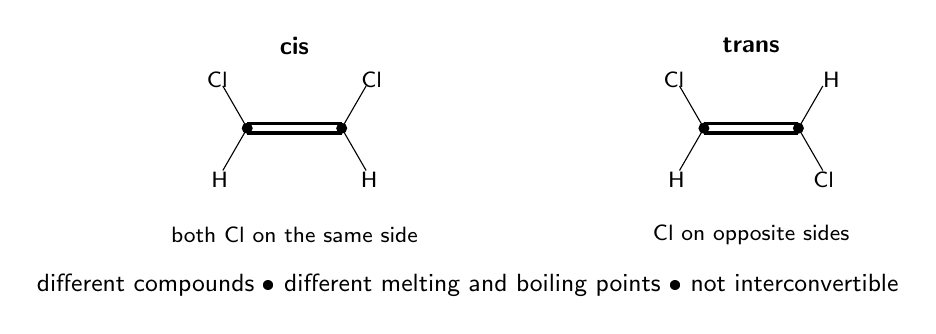
\begin{tikzpicture}[font=\sffamily\footnotesize]
  % cis
  \node[font=\sffamily\small\bfseries] at (1.4,2.05) {\emph{cis}};
  \fill (0.8,1.0) circle (0.07); \fill (2.0,1.0) circle (0.07);
  \draw[very thick] (0.8,1.06) -- (2.0,1.06);
  \draw[very thick] (0.8,0.94) -- (2.0,0.94);
  \draw (0.8,1.0) -- ++(120:0.62); \node at (0.42,1.62) {Cl};
  \draw (2.0,1.0) -- ++(60:0.62);  \node at (2.38,1.62) {Cl};
  \draw (0.8,1.0) -- ++(240:0.62); \node at (0.45,0.34) {H};
  \draw (2.0,1.0) -- ++(300:0.62); \node at (2.35,0.34) {H};
  \node at (1.4,-0.35) {both Cl on the same side};

  % trans
  \begin{scope}[xshift=5.8cm]
    \node[font=\sffamily\small\bfseries] at (1.4,2.05) {\emph{trans}};
    \fill (0.8,1.0) circle (0.07); \fill (2.0,1.0) circle (0.07);
    \draw[very thick] (0.8,1.06) -- (2.0,1.06);
    \draw[very thick] (0.8,0.94) -- (2.0,0.94);
    \draw (0.8,1.0) -- ++(120:0.62); \node at (0.42,1.62) {Cl};
    \draw (2.0,1.0) -- ++(60:0.62);  \node at (2.42,1.62) {H};
    \draw (0.8,1.0) -- ++(240:0.62); \node at (0.45,0.34) {H};
    \draw (2.0,1.0) -- ++(300:0.62); \node at (2.32,0.34) {Cl};
    \node at (1.4,-0.35) {Cl on opposite sides};
  \end{scope}
  \node[font=\sffamily\small,align=center] at (3.6,-1.0)
    {different compounds \textbullet\ different melting and boiling
     points \textbullet\ not interconvertible};
\end{tikzpicture}
\end{center}

\begin{workedexample}[I do: why one has isomers and the other does not]
\textbf{\ce{C2H4Cl2} with a single \ce{C-C} bond} ---
1,2-dichloroethane. The \ce{C-C} bond is a lone $\sigma$, cylindrically
symmetric, so the two \ce{CH2Cl} ends spin freely at room temperature.
Any arrangement converts into any other billions of times a second, so
there is only \textbf{one} compound.

\textbf{\ce{C2H2Cl2} with a double \ce{C=C} bond} ---
1,2-dichloroethene. Now the $\pi$ bond holds the two ends rigidly
coplanar. Turning one end over would require breaking the sideways $p$
overlap, which costs far more energy than is available at room
temperature.

So the two chlorines are stuck either on the same side (\emph{cis}) or
on opposite sides (\emph{trans}), and these are \textbf{two different
compounds} with different physical properties --- different melting
points, different boiling points, different dipole moments (\emph{cis}
is polar, \emph{trans} is not).

\textbf{The general statement:} $\pi$ bonds lock geometry. That single
fact explains \emph{cis}/\emph{trans} isomerism, why fats are described
as \emph{cis}-unsaturated, and how vision works --- the retinal molecule
in your eye responds to light by flipping one \emph{cis} double bond to
\emph{trans}.
\end{workedexample}

\begin{yourturn}[YOUR TURN 7 --- four questions]
\begin{enumerate}[leftmargin=*,itemsep=0.5em]
  \item Can \ce{H3C-CH3} show \emph{cis}/\emph{trans} isomerism?
        Explain. \workspace[1.6cm]
  \item Which bond in a double bond must break to allow rotation?
        \workspace[1.4cm]
  \item Of \emph{cis}- and \emph{trans}-1,2-dichloroethene, which is
        polar? \workspace[1.6cm]
  \item Why can a triple bond not show \emph{cis}/\emph{trans}
        isomerism? \workspace[1.8cm]
\end{enumerate}
\selfcheck{(a) no --- free rotation about the $\sigma$ \quad (b) the
$\pi$ \quad (c) \emph{cis} \quad (d) it is linear, so there are no
``sides''}
\keyonly{\begin{apcanswer}(a) \textbf{No.} The \ce{C-C} bond is a single
$\sigma$ bond, and rotation about it is free, so all arrangements are
the same compound. (b) The \textbf{$\pi$ bond}. The $\sigma$ survives
rotation --- it is cylindrically symmetric --- but the sideways $p$
overlap of the $\pi$ is destroyed. (c) \textbf{\emph{cis}}. Its two
\ce{C-Cl} dipoles point to the same side and partly add;
in \emph{trans} they point oppositely and cancel, so \emph{trans} is
nonpolar. (d) A triple-bonded carbon is \textbf{$sp$} and therefore
\textbf{linear}: the two remaining substituents lie on the bond axis
itself, one at each end. There is no ``same side'' or ``opposite side''
for them to occupy.\end{apcanswer}}
\end{yourturn}

% =====================================================================
\section*{\sffamily Ladder 8 \textbullet\ Full analysis of a molecule}
\zsec{9.1}

Everything from Ladders 1--7, applied in one pass. The order never
changes:

\begin{center}
\fbox{\parbox{0.93\linewidth}{\centering
Lewis structure $\to$ count domains on \emph{each} interior atom $\to$
hybridization $\to$ geometry and angles $\to$ count $\sigma$ and $\pi$}}
\end{center}

\begin{workedexample}[I do: acetic acid, \ce{CH3COOH}]
The skeleton is \ce{CH3-C(=O)-O-H}. Take the interior atoms one at a
time.

\textbf{Methyl carbon.} Four single bonds $=$ 4 domains $\Rightarrow$
\textbf{$sp^{3}$}, tetrahedral, \SI{109.5}{\degree}.

\textbf{Carbonyl carbon.} One \ce{C=O} $+$ two single bonds $=$
3 domains $\Rightarrow$ \textbf{$sp^{2}$}, trigonal planar,
\SI{120}{\degree}.

\textbf{Carbonyl oxygen} (the double-bonded one). One double bond $+$
two lone pairs $=$ 3 domains $\Rightarrow$ \textbf{$sp^{2}$}.

\textbf{Hydroxyl oxygen.} Two single bonds $+$ two lone pairs $=$
4 domains $\Rightarrow$ \textbf{$sp^{3}$}, bent at the oxygen.

\textbf{Bond count.} Every single bond is one $\sigma$; the one double
bond adds a $\pi$. Three \ce{C-H}, one \ce{C-C}, one \ce{C=O} $\sigma$,
one \ce{C-O} $\sigma$, one \ce{O-H} $=$
\[ \mathbf{7~\sigma \;+\; 1~\pi} \]

\textbf{What this molecule demonstrates.} \emph{Four} interior atoms,
\emph{three} different hybridizations, and two oxygens that differ from
each other. A question asking only for ``the hybridization of the
central atom'' would be meaningless here --- which is why the procedure
works atom by atom.
\end{workedexample}

\begin{yourturn}[YOUR TURN 8 --- four questions]
Consider acetonitrile, \ce{CH3CN} (skeleton \ce{H3C-C#N}).
\begin{enumerate}[leftmargin=*,itemsep=0.5em]
  \item Hybridization of the methyl carbon. \workspace[1.4cm]
  \item Hybridization of the nitrile carbon and of the nitrogen.
        \workspace[1.6cm]
  \item Total $\sigma$ and $\pi$ bonds in the molecule.
        \workspace[1.6cm]
  \item Give the approximate \ce{H-C-H} angle and the \ce{C-C#N} angle.
        \workspace[1.6cm]
\end{enumerate}
\selfcheck{(a) $sp^{3}$ \quad (b) both $sp$ \quad (c) 5 $\sigma$, 2
$\pi$ \quad (d) \SI{109.5}{\degree} and \SI{180}{\degree}}
\keyonly{\begin{apcanswer}(a) Four single bonds $=$ 4 domains:
\textbf{$sp^{3}$}. (b) Nitrile carbon: one single $+$ one triple $=$
2 domains $\Rightarrow$ \textbf{$sp$}. Nitrogen: one triple $+$ one lone
pair $=$ 2 domains $\Rightarrow$ \textbf{$sp$}. (c) Three \ce{C-H}
$\sigma$, one \ce{C-C} $\sigma$, one \ce{C-N} $\sigma$, plus two $\pi$
from the triple bond: \textbf{5 $\sigma$ and 2 $\pi$}. (d) At the
$sp^{3}$ methyl carbon, \ce{H-C-H} is about
\textbf{\SI{109.5}{\degree}}; at the $sp$ nitrile carbon the
\ce{C-C#N} arrangement is \textbf{\SI{180}{\degree}} --- so one molecule
carries both a tetrahedral corner and a linear
segment.\end{apcanswer}}
\end{yourturn}

% =====================================================================
\section*{\sffamily Ladder 9 \textbullet\ ENRICHMENT: molecular orbitals}
\zsec{9.2--9.3}

\begin{apctrap}
\textbf{Not on the AP CED.} Molecular orbital theory was dropped in the
2019 redesign, and no AP question will ask for an MO diagram, an MO bond
order, or the electron configuration of \ce{O2} in MO terms. This ladder
exists because MO explains one thing the localized model gets plainly
wrong, and because it is standard in college chemistry. \textbf{Skip it
with a clear conscience if you are short of time.}
\end{apctrap}

Two atomic orbitals combine into two molecular orbitals: one
\textbf{bonding} (lower energy, density between the nuclei) and one
\textbf{antibonding} (higher, with a node between them).

\[ \text{bond order} =
   \frac{(\text{bonding e}^-) - (\text{antibonding e}^-)}{2} \]

\begin{center}
\begin{tikzpicture}[font=\sffamily\footnotesize]
  % O2 MO sketch (valence only, simplified)
  \node[font=\sffamily\small\bfseries] at (2.6,3.5) {\ce{O2}: valence MOs
    (simplified)};
  \foreach \y/\lab in {0.2/{$\sigma_{2s}$}, 0.85/{$\sigma^{*}_{2s}$},
                       1.5/{$\sigma_{2p}$}, 2.15/{$\pi_{2p}$},
                       2.8/{$\pi^{*}_{2p}$}} {
    \draw[thick] (2.1,\y) -- (3.1,\y);
    \node[right] at (3.25,\y) {\lab};}
  % second pi level
  \draw[thick] (1.0,2.15) -- (2.0,2.15);
  \draw[thick] (1.0,2.8) -- (2.0,2.8);
  % electrons: paired arrows
  \foreach \y in {0.2,0.85,1.5} {
    \draw[-{Stealth[length=1.6mm]}] (2.45,\y-0.16) -- (2.45,\y+0.16);
    \draw[-{Stealth[length=1.6mm]}] (2.75,\y+0.16) -- (2.75,\y-0.16);}
  \foreach \x in {1.5,2.6} {
    \draw[-{Stealth[length=1.6mm]}] (\x-0.15,2.15-0.16) -- (\x-0.15,2.15+0.16);
    \draw[-{Stealth[length=1.6mm]}] (\x+0.15,2.15+0.16) -- (\x+0.15,2.15-0.16);}
  % the two unpaired pi* electrons
  \draw[-{Stealth[length=1.6mm]},very thick] (1.5,2.8-0.16) -- (1.5,2.8+0.16);
  \draw[-{Stealth[length=1.6mm]},very thick] (2.6,2.8-0.16) -- (2.6,2.8+0.16);
  \node[align=left,font=\sffamily\footnotesize] at (6.6,2.8)
    {two \textbf{unpaired} electrons};
  \node[align=left,font=\sffamily\footnotesize] at (6.9,1.2)
    {bonding 8, antibonding 4\\
     bond order $= (8-4)/2 = \mathbf{2}$};
  % 'energy' sits BESIDE the arrow, rotated -- as a node[above] on the
  % arrow tip it printed straight through the figure title.
  \draw[-{Stealth[length=2.4mm]}] (0.4,0.1) -- (0.4,3.1);
  \node[rotate=90,font=\sffamily\footnotesize] at (0.1,1.6) {energy};
\end{tikzpicture}
\end{center}

\begin{workedexample}[I do: the one thing Lewis structures get wrong]
\textbf{Draw the Lewis structure of \ce{O2}.} You get \ce{O=O} with two
lone pairs on each oxygen --- every electron paired.

\textbf{Now measure it.} Liquid oxygen is \textbf{paramagnetic}: poured
between the poles of a magnet, it sticks. Paramagnetism requires
\emph{unpaired} electrons, and the Lewis structure has none. The
localized model is simply wrong here.

\textbf{What MO theory says.} Filling the valence molecular orbitals for
\ce{O2}'s 12 valence electrons puts the last two in \emph{different}
$\pi^{*}$ orbitals with parallel spins --- Hund's rule again. Two
unpaired electrons, exactly as the magnet shows.

\textbf{And the bond order still comes out right:}
\[ \frac{8 - 4}{2} = 2 \]
a double bond, agreeing with Lewis on the bond strength while
disagreeing about the spins.

\textbf{The lesson worth keeping even though this is off-syllabus:} a
model is a tool, not the truth. The localized model handles geometry
beautifully and paramagnetism not at all; MO does the reverse. Chemists
use whichever answers the question in front of them.
\end{workedexample}

\begin{yourturn}[YOUR TURN 9 --- four questions, enrichment only]
\begin{enumerate}[leftmargin=*,itemsep=0.5em]
  \item \ce{N2} has 10 valence electrons: 8 bonding, 2 antibonding. Give
        the bond order. \workspace[1.4cm]
  \item Is \ce{N2} paramagnetic or diamagnetic? \workspace[1.4cm]
  \item What does a bond order of zero imply about a species?
        \workspace[1.4cm]
  \item State one thing the localized model does better than MO theory.
        \workspace[1.6cm]
\end{enumerate}
\selfcheck{(a) 3 \quad (b) diamagnetic --- all paired \quad (c) it does
not exist as a stable molecule \quad (d) predicting molecular geometry}
\keyonly{\begin{apcanswer}(a) $(8-2)/2 = \mathbf{3}$ --- a triple bond,
consistent with \ce{N2}'s enormous bond energy of 941 kJ/mol.
(b) \textbf{Diamagnetic}: all ten valence electrons are paired, so
\ce{N2} is weakly repelled by a magnetic field rather than attracted.
(c) That the bonding and antibonding electrons exactly cancel, so there
is \textbf{no net bond} and the species does not exist as a stable
molecule --- which is why \ce{He2} is not found. (d) \textbf{Molecular
geometry.} Hybridization and VSEPR predict shapes and bond angles
directly and easily; MO diagrams for polyatomic molecules become
complicated fast and are not how shapes are
predicted.\end{apcanswer}}
\end{yourturn}

% =====================================================================
\section*{\sffamily Mastery tracker}

Tick a row only if \textbf{all four} YOUR TURN questions were right on
the first attempt. Ladder 9 is enrichment --- an untickable row there
costs you nothing.

\renewcommand{\arraystretch}{1.35}
\noindent\begin{tabular}{@{}c p{6.2cm} c p{4.8cm}@{}}
\toprule
\textbf{First try?} & \textbf{Skill} & \textbf{Ladder} &
  \textbf{If not, re-read\ldots}\\
\midrule
$\square$ & why hybridization exists & 1 & orbitals in $=$ orbitals out \\
$\square$ & domains to hybridization & 2 & domains, not bonds \\
$\square$ & sigma and pi bonds & 3 & one $\sigma$ per bond, rest $\pi$ \\
$\square$ & $sp^{3}$ and lone pairs & 4 & hybrid vs molecular shape \\
$\square$ & $sp^{2}$ and the pi bond & 5 & the leftover $p$ \\
$\square$ & $sp$ and two pi bonds & 6 & two leftover $p$ \\
$\square$ & restricted rotation, isomers & 7 & $\pi$ locks geometry \\
$\square$ & full molecular analysis & 8 & every interior atom \\
\midrule
\textit{(opt.)} & molecular orbitals & 9 & \textit{not assessed} \\
\bottomrule
\end{tabular}

\begin{apcnote}[Scoring yourself honestly]
8/8 on Ladders 1--8: you have Chapter 9's assessed content. It is a
short chapter by AP standards precisely because most of Zumdahl's
Chapter 9 is off-syllabus --- do not mistake its brevity for
unimportance, because hybridization appears on nearly every structure
question.

6--7: redo the missed ladders tomorrow, not today.

5 or fewer: the misses are almost certainly in Ladder 2, and everything
downstream inherits them. Go back and practise counting
\textbf{domains} on twenty Lewis structures --- double and triple bonds
as one, lone pairs as one each --- until the count is automatic. Every
other ladder in this chapter is built on that single skill.
\end{apcnote}

\end{document}
